\subsection{Описание предложенного подхода}
Для решения задачи, поставленной в пункте~\ref{formulation} в данной работе предлагается подход, основанный на введении в облачную систему дополнительного сервиса как показано на рис.~\ref{suggested-approach}.
Такой сервис будет называться далее сервисом управления виртуализированной инфраструктурой.

\begin{figure}[hbtp]
    \centering
    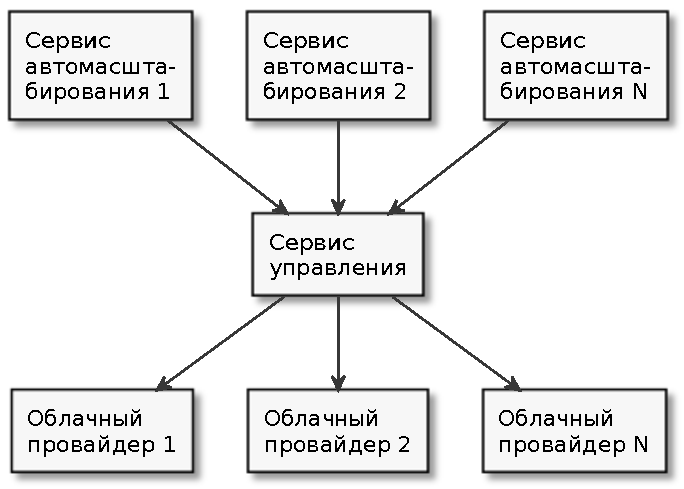
\includegraphics[width=10cm]{img/suggested-approach.pdf}
    \caption{Облачная система с дополнительным сервисом управления}
    \label{suggested-approach}
\end{figure}

При помощи введения в систему дополнительного промежуточного компонента решается задача абстрагирования компонентов управления ресурсами от конкретных объектов управления - платформ виртуализации инфраструктуры. 
Таким образом, при разработке компонента управления ресурсами (например, сервиса автомасштабирования), нужно будет учитывать только программный интерфейс (API) сервиса управления, даже если в целевой системе будет несколько различных платформ облачных вычислений.

Тем не менее, при необходимости введения в систему новой платформы виртуализации, возникнет необходимость доработки сервиса управления с учётом программного интерфейса добавляемой платформы.
Однако это потребуется сделать лишь один раз и далее можно будет использовать неограниченное количество облачных платформ, предоставляющих такой же программный интерфейс.

